
%% bare_jrnl.tex
%% V1.4b
%% 2015/08/26
%% by Michael Shell
%% see http://www.michaelshell.org/
%% for current contact information.
%%
%% This is a skeleton file demonstrating the use of IEEEtran.cls
%% (requires IEEEtran.cls version 1.8b or later) with an IEEE
%% journal paper.
%%
%% Support sites:
%% http://www.michaelshell.org/tex/ieeetran/
%% http://www.ctan.org/pkg/ieeetran
%% and
%% http://www.ieee.org/



%%*************************************************************************
%% Legal Notice:
%% This code is offered as-is without any warranty either expressed or
%% implied; without even the implied warranty of MERCHANTABILITY or
%% FITNESS FOR A PARTICULAR PURPOSE! 
%% User assumes all risk.
%% In no event shall the IEEE or any contributor to this code be liable for
%% any damages or losses, including, but not limited to, incidental,
%% consequential, or any other damages, resulting from the use or misuse
%% of any information contained here.
%%
%% All comments are the opinions of their respective authors and are not
%% necessarily endorsed by the IEEE.
%%
%% This work is distributed under the LaTeX Project Public License (LPPL)
%% ( http://www.latex-project.org/ ) version 1.3, and may be freely used,
%% distributed and modified. A copy of the LPPL, version 1.3, is included
%% in the base LaTeX documentation of all distributions of LaTeX released
%% 2003/12/01 or later.
%% Retain all contribution notices and credits.
%% ** Modified files should be clearly indicated as such, including  **
%% ** renaming them and changing author support contact information. **
%%*************************************************************************


% *** Authors should verify (and, if needed, correct) their LaTeX system  ***
% *** with the testflow diagnostic prior to trusting their LaTeX platform ***
% *** with production work. The IEEE's font choices and paper sizes can   ***
% *** trigger bugs that do not appear when using other class files.       ***                          ***
% The testflow support page is at:
% http://www.michaelshell.org/tex/testflow/


\documentclass[journal]{IEEEtran}
%
% If IEEEtran.cls has not been installed into the LaTeX system files,
% manually specify the path to it like:
% \documentclass[journal]{../sty/IEEEtran}

\usepackage{graphicx}




% Some very useful LaTeX packages include:
% (uncomment the ones you want to load)


% *** MISC UTILITY PACKAGES ***
%
%\usepackage{ifpdf}
% Heiko Oberdiek's ifpdf.sty is very useful if you need conditional
% compilation based on whether the output is pdf or dvi.
% usage:
% \ifpdf
%   % pdf code
% \else
%   % dvi code
% \fi
% The latest version of ifpdf.sty can be obtained from:
% http://www.ctan.org/pkg/ifpdf
% Also, note that IEEEtran.cls V1.7 and later provides a builtin
% \ifCLASSINFOpdf conditional that works the same way.
% When switching from latex to pdflatex and vice-versa, the compiler may
% have to be run twice to clear warning/error messages.






% *** CITATION PACKAGES ***
%
%\usepackage{cite}
% cite.sty was written by Donald Arseneau
% V1.6 and later of IEEEtran pre-defines the format of the cite.sty package
% \cite{} output to follow that of the IEEE. Loading the cite package will
% result in citation numbers being automatically sorted and properly
% "compressed/ranged". e.g., [1], [9], [2], [7], [5], [6] without using
% cite.sty will become [1], [2], [5]--[7], [9] using cite.sty. cite.sty's
% \cite will automatically add leading space, if needed. Use cite.sty's
% noadjust option (cite.sty V3.8 and later) if you want to turn this off
% such as if a citation ever needs to be enclosed in parenthesis.
% cite.sty is already installed on most LaTeX systems. Be sure and use
% version 5.0 (2009-03-20) and later if using hyperref.sty.
% The latest version can be obtained at:
% http://www.ctan.org/pkg/cite
% The documentation is contained in the cite.sty file itself.






% *** GRAPHICS RELATED PACKAGES ***
%
\ifCLASSINFOpdf
  % \usepackage[pdftex]{graphicx}
  % declare the path(s) where your graphic files are
  % \graphicspath{{../pdf/}{../jpeg/}}
  % and their extensions so you won't have to specify these with
  % every instance of \includegraphics
  % \DeclareGraphicsExtensions{.pdf,.jpeg,.png}
\else
  % or other class option (dvipsone, dvipdf, if not using dvips). graphicx
  % will default to the driver specified in the system graphics.cfg if no
  % driver is specified.
  % \usepackage[dvips]{graphicx}
  % declare the path(s) where your graphic files are
  % \graphicspath{{../eps/}}
  % and their extensions so you won't have to specify these with
  % every instance of \includegraphics
  % \DeclareGraphicsExtensions{.eps}
\fi
% graphicx was written by David Carlisle and Sebastian Rahtz. It is
% required if you want graphics, photos, etc. graphicx.sty is already
% installed on most LaTeX systems. The latest version and documentation
% can be obtained at: 
% http://www.ctan.org/pkg/graphicx
% Another good source of documentation is "Using Imported Graphics in
% LaTeX2e" by Keith Reckdahl which can be found at:
% http://www.ctan.org/pkg/epslatex
%
% latex, and pdflatex in dvi mode, support graphics in encapsulated
% postscript (.eps) format. pdflatex in pdf mode supports graphics
% in .pdf, .jpeg, .png and .mps (metapost) formats. Users should ensure
% that all non-photo figures use a vector format (.eps, .pdf, .mps) and
% not a bitmapped formats (.jpeg, .png). The IEEE frowns on bitmapped formats
% which can result in "jaggedy"/blurry rendering of lines and letters as
% well as large increases in file sizes.
%
% You can find documentation about the pdfTeX application at:
% http://www.tug.org/applications/pdftex





% *** MATH PACKAGES ***
%
%\usepackage{amsmath}
% A popular package from the American Mathematical Society that provides
% many useful and powerful commands for dealing with mathematics.
%
% Note that the amsmath package sets \interdisplaylinepenalty to 10000
% thus preventing page breaks from occurring within multiline equations. Use:
%\interdisplaylinepenalty=2500
% after loading amsmath to restore such page breaks as IEEEtran.cls normally
% does. amsmath.sty is already installed on most LaTeX systems. The latest
% version and documentation can be obtained at:
% http://www.ctan.org/pkg/amsmath





% *** SPECIALIZED LIST PACKAGES ***
%
%\usepackage{algorithmic}
% algorithmic.sty was written by Peter Williams and Rogerio Brito.
% This package provides an algorithmic environment fo describing algorithms.
% You can use the algorithmic environment in-text or within a figure
% environment to provide for a floating algorithm. Do NOT use the algorithm
% floating environment provided by algorithm.sty (by the same authors) or
% algorithm2e.sty (by Christophe Fiorio) as the IEEE does not use dedicated
% algorithm float types and packages that provide these will not provide
% correct IEEE style captions. The latest version and documentation of
% algorithmic.sty can be obtained at:
% http://www.ctan.org/pkg/algorithms
% Also of interest may be the (relatively newer and more customizable)
% algorithmicx.sty package by Szasz Janos:
% http://www.ctan.org/pkg/algorithmicx




% *** ALIGNMENT PACKAGES ***
%
%\usepackage{array}
% Frank Mittelbach's and David Carlisle's array.sty patches and improves
% the standard LaTeX2e array and tabular environments to provide better
% appearance and additional user controls. As the default LaTeX2e table
% generation code is lacking to the point of almost being broken with
% respect to the quality of the end results, all users are strongly
% advised to use an enhanced (at the very least that provided by array.sty)
% set of table tools. array.sty is already installed on most systems. The
% latest version and documentation can be obtained at:
% http://www.ctan.org/pkg/array


% IEEEtran contains the IEEEeqnarray family of commands that can be used to
% generate multiline equations as well as matrices, tables, etc., of high
% quality.




% *** SUBFIGURE PACKAGES ***
%\ifCLASSOPTIONcompsoc
%  \usepackage[caption=false,font=normalsize,labelfont=sf,textfont=sf]{subfig}
%\else
%  \usepackage[caption=false,font=footnotesize]{subfig}
%\fi
% subfig.sty, written by Steven Douglas Cochran, is the modern replacement
% for subfigure.sty, the latter of which is no longer maintained and is
% incompatible with some LaTeX packages including fixltx2e. However,
% subfig.sty requires and automatically loads Axel Sommerfeldt's caption.sty
% which will override IEEEtran.cls' handling of captions and this will result
% in non-IEEE style figure/table captions. To prevent this problem, be sure
% and invoke subfig.sty's "caption=false" package option (available since
% subfig.sty version 1.3, 2005/06/28) as this is will preserve IEEEtran.cls
% handling of captions.
% Note that the Computer Society format requires a larger sans serif font
% than the serif footnote size font used in traditional IEEE formatting
% and thus the need to invoke different subfig.sty package options depending
% on whether compsoc mode has been enabled.
%
% The latest version and documentation of subfig.sty can be obtained at:
% http://www.ctan.org/pkg/subfig




% *** FLOAT PACKAGES ***
%
%\usepackage{fixltx2e}
% fixltx2e, the successor to the earlier fix2col.sty, was written by
% Frank Mittelbach and David Carlisle. This package corrects a few problems
% in the LaTeX2e kernel, the most notable of which is that in current
% LaTeX2e releases, the ordering of single and double column floats is not
% guaranteed to be preserved. Thus, an unpatched LaTeX2e can allow a
% single column figure to be placed prior to an earlier double column
% figure.
% Be aware that LaTeX2e kernels dated 2015 and later have fixltx2e.sty's
% corrections already built into the system in which case a warning will
% be issued if an attempt is made to load fixltx2e.sty as it is no longer
% needed.
% The latest version and documentation can be found at:
% http://www.ctan.org/pkg/fixltx2e


%\usepackage{stfloats}
% stfloats.sty was written by Sigitas Tolusis. This package gives LaTeX2e
% the ability to do double column floats at the bottom of the page as well
% as the top. (e.g., "\begin{figure*}[!b]" is not normally possible in
% LaTeX2e). It also provides a command:
%\fnbelowfloat
% to enable the placement of footnotes below bottom floats (the standard
% LaTeX2e kernel puts them above bottom floats). This is an invasive package
% which rewrites many portions of the LaTeX2e float routines. It may not work
% with other packages that modify the LaTeX2e float routines. The latest
% version and documentation can be obtained at:
% http://www.ctan.org/pkg/stfloats
% Do not use the stfloats baselinefloat ability as the IEEE does not allow
% \baselineskip to stretch. Authors submitting work to the IEEE should note
% that the IEEE rarely uses double column equations and that authors should try
% to avoid such use. Do not be tempted to use the cuted.sty or midfloat.sty
% packages (also by Sigitas Tolusis) as the IEEE does not format its papers in
% such ways.
% Do not attempt to use stfloats with fixltx2e as they are incompatible.
% Instead, use Morten Hogholm'a dblfloatfix which combines the features
% of both fixltx2e and stfloats:
%
% \usepackage{dblfloatfix}
% The latest version can be found at:
% http://www.ctan.org/pkg/dblfloatfix




%\ifCLASSOPTIONcaptionsoff
%  \usepackage[nomarkers]{endfloat}
% \let\MYoriglatexcaption\caption
% \renewcommand{\caption}[2][\relax]{\MYoriglatexcaption[#2]{#2}}
%\fi
% endfloat.sty was written by James Darrell McCauley, Jeff Goldberg and 
% Axel Sommerfeldt. This package may be useful when used in conjunction with 
% IEEEtran.cls'  captionsoff option. Some IEEE journals/societies require that
% submissions have lists of figures/tables at the end of the paper and that
% figures/tables without any captions are placed on a page by themselves at
% the end of the document. If needed, the draftcls IEEEtran class option or
% \CLASSINPUTbaselinestretch interface can be used to increase the line
% spacing as well. Be sure and use the nomarkers option of endfloat to
% prevent endfloat from "marking" where the figures would have been placed
% in the text. The two hack lines of code above are a slight modification of
% that suggested by in the endfloat docs (section 8.4.1) to ensure that
% the full captions always appear in the list of figures/tables - even if
% the user used the short optional argument of \caption[]{}.
% IEEE papers do not typically make use of \caption[]'s optional argument,
% so this should not be an issue. A similar trick can be used to disable
% captions of packages such as subfig.sty that lack options to turn off
% the subcaptions:
% For subfig.sty:
% \let\MYorigsubfloat\subfloat
% \renewcommand{\subfloat}[2][\relax]{\MYorigsubfloat[]{#2}}
% However, the above trick will not work if both optional arguments of
% the \subfloat command are used. Furthermore, there needs to be a
% description of each subfigure *somewhere* and endfloat does not add
% subfigure captions to its list of figures. Thus, the best approach is to
% avoid the use of subfigure captions (many IEEE journals avoid them anyway)
% and instead reference/explain all the subfigures within the main caption.
% The latest version of endfloat.sty and its documentation can obtained at:
% http://www.ctan.org/pkg/endfloat
%
% The IEEEtran \ifCLASSOPTIONcaptionsoff conditional can also be used
% later in the document, say, to conditionally put the References on a 
% page by themselves.




% *** PDF, URL AND HYPERLINK PACKAGES ***
%
%\usepackage{url}
% url.sty was written by Donald Arseneau. It provides better support for
% handling and breaking URLs. url.sty is already installed on most LaTeX
% systems. The latest version and documentation can be obtained at:
% http://www.ctan.org/pkg/url
% Basically, \url{my_url_here}.




% *** Do not adjust lengths that control margins, column widths, etc. ***
% *** Do not use packages that alter fonts (such as pslatex).         ***
% There should be no need to do such things with IEEEtran.cls V1.6 and later.
% (Unless specifically asked to do so by the journal or conference you plan
% to submit to, of course. )


% correct bad hyphenation here
\hyphenation{op-tical net-works semi-conduc-tor}
\begin{document}
%
% paper title
% Titles are generally capitalized except for words such as a, an, and, as,
% at, but, by, for, in, nor, of, on, or, the, to and up, which are usually
% not capitalized unless they are the first or last word of the title.
\title{Arrhythmia Heartbeat Classification Using \\Deep Learning Hybrid Structure with Massive Unannotated Electrocardiography Samples}
%
% author names and IEEE memberships
% note positions of commas and nonbreaking spaces ( ~ ) LaTeX will not break
% a structure at a ~ so this keeps an author's name from being broken across
% two lines.
% use \thanks{} to gain access to the first footnote area
% a separate \thanks must be used for each paragraph as LaTeX2e's \thanks
% was not built to handle multiple paragraphs
%

\author{Yan~Yan,~\IEEEmembership{Student Member, IEEE},
        and~Lei~Wang~% <-this % stops a space
\thanks{Y. Yan is with the Shenzhen Key Laboratory for Low-cost Healthcare, Shenzhen Institutes of Advanced Technology, Chinese Academy of Sciences. No. 1068, Xueyuan Road, Nanshan District,
Shenzhen, Guangdong Province, China-mail: (yan.yan@siat.ac.cn).}% <-this % stops a space
\thanks{X. Qin is with the Shenzhen Institutes of Advanced Technology, Chinese Academy of Sciences.
No. 1068, Xueyuan Road, Nanshan District, Shenzhen, Guangdong Province, China.}% <-this % stops a space
\thanks{J. Fan is with the Shenzhen Institutes of Advanced Technology, Chinese Academy of Sciences. No. 1068, Xueyuan Road, Nanshan District, Shenzhen, Guangdong Province, China.}% <-this % stops a space
\thanks{L. Wang is with the Shenzhen Key Laboratory for Low-cost Healthcare, Shenzhen Institutes of Advanced Technology, Chinese Academy of Sciences.
No. 1068, Xueyuan Road, Nanshan District,
Shenzhen, Guangdong Province, China.}% <-this % stops a space
\thanks{Manuscript received ; }}

% note the % following the last \IEEEmembership and also \thanks - 
% these prevent an unwanted space from occurring between the last author name
% and the end of the author line. i.e., if you had this:
% 
% \author{....lastname \thanks{...} \thanks{...} }
%                     ^------------^------------^----Do not want these spaces!
%
% a space would be appended to the last name and could cause every name on that
% line to be shifted left slightly. This is one of those "LaTeX things". For
% instance, "\textbf{A} \textbf{B}" will typeset as "A B" not "AB". To get
% "AB" then you have to do: "\textbf{A}\textbf{B}"
% \thanks is no different in this regard, so shield the last } of each \thanks
% that ends a line with a % and do not let a space in before the next \thanks.
% Spaces after \IEEEmembership other than the last one are OK (and needed) as
% you are supposed to have spaces between the names. For what it is worth,
% this is a minor point as most people would not even notice if the said evil
% space somehow managed to creep in.



% The paper headers
\markboth{IEEE Transactions on Biomedical Engineering,~Vol.~, No.~, April ~2016}%
{Shell \MakeLowercase{\textit{et al.}}: }
% The only time the second header will appear is for the odd numbered pages
% after the title page when using the twoside option.
% 
% *** Note that you probably will NOT want to include the author's ***
% *** name in the headers of peer review papers.                   ***
% You can use \ifCLASSOPTIONpeerreview for conditional compilation here if
% you desire.


% If you want to put a publisher's ID mark on the page you can do it like
% this:
%\IEEEpubid{0000--0000/00\$00.00~\copyright~2015 IEEE}
% Remember, if you use this you must call \IEEEpubidadjcol in the second
% column for its text to clear the IEEEpubid mark.



% use for special paper notices
%\IEEEspecialpapernotice{(Invited Paper)}




% make the title area
\maketitle

% As a general rule, do not put math, special symbols or citations
% in the abstract or keywords.
\begin{abstract}

Plenty of samples with the diagnosis can be used to improve the CAD systems' performance. 
These ECG signal samples were able to be easily acquired from routine medical examinations or Holter monitoring applications. 
However, making annotations one by one for the massive ECG signal samples could be time-consuming and inefficient, which would bring heavy burden for medical experts. 
In the mobile healthcare or e-healthcare applications, the medical experts based ECG analysis method would be impossible to handle the growing data from the large user population.

\end{abstract}

% Note that keywords are not normally used for peer review papers.
\begin{IEEEkeywords}
ECG Classification, Deep Learning, Arrythmia Analysis
\end{IEEEkeywords}


% For peer review papers, you can put extra information on the cover
% page as needed:
 \ifCLASSOPTIONpeerreview
 \begin{center} \bfseries EDICS Category: 3-BBND \end{center}
 \fi
%
% For peerreview papers, this IEEEtran command inserts a page break and
% creates the second title. It will be ignored for other modes.
\IEEEpeerreviewmaketitle



\section{Introduction}


% The very first letter is a 2 line initial drop letter followed
% by the rest of the first word in caps.
% 
% form to use if the first word consists of a single letter:
% \IEEEPARstart{A}{demo} file is ....
% 
% form to use if you need the single drop letter followed by
% normal text (unknown if ever used by the IEEE):
% \IEEEPARstart{A}{}demo file is ....
% 
% Some journals put the first two words in caps:
% \IEEEPARstart{T}{his demo} file is ....
% 
% Here we have the typical use of a "T" for an initial drop letter
% and "HIS" in caps to complete the first word.
\IEEEPARstart{T}{}{he} research of the electrocardiogram (ECG) signal provides valuable insights for cardiac function and condition understandings.
Heart function analysis is of particular concern in the diagnosis of cardiovascular disease. 
The ECG computer-aided diagnosis (CAD) systems provide indispensable assist in long-term clinical monitoring, and a large number of approaches had been proposed for the task, easing the determination of arrhythmic changes as well as further inspection, e.g., heart rate variability or heart turbulence analysis\cite{mar2011}. As the wearable techniques promoted the accumulation of ECG data from personal and mobile healthcare applications, the automated ECG signal analysis techniques featured CAD systems tend to be more important \cite{jankowski2003, winokur2013}.
Machine learning techniques had been widely used in data analysis and applied in ECG-CAD systems.
These methods learn representations from the diagnosed samples collected from medical examinations, to assist the decision making of medical experts.

Plenty of samples with the diagnosis can be used to improve the CAD systems' performance. 
These ECG signal samples were able to be easily acquired from routine medical examinations or Holter monitoring applications. 
However, making annotations one by one for the massive ECG signal samples could be time-consuming and inefficient, which would bring heavy burden for medical experts. 
In the mobile healthcare or e-healthcare applications, the medical experts based ECG analysis method would be impossible to handle the growing data from the large user population.

The possible solution for massive ECG automated analysis is to learn hypothesis from a few of samples annotated by medical experts (the labeled data) and then utilize the massive undiagnosed samples (the unlabeled data) to enhance the performance of the learned hypothesis.
In machine learning, this technique is called learning with labeled (supervised learning) and unlabeled data (unsupervised learning).
While the semi-supervised learning method could enhance the performance of the learned hypothesis by using the labeled and unlabeled data together.
Deep learning is one kind of machine learning methods which becomes quite popular in recent research in computer vision and acoustic signal analysis applications. Deep learning refers to a rather broad class of machine learning techniques and architectures, with the hallmark of using many layers of non-linear information processing that are hierarchical in nature \cite{deng2014deeplearning} . 

The results from the intelligent algorithms or models were not amenable to expert labelling, as well as for the identification of complex relationships between subjects and clinical conditions \cite{clifford2006}. But for the ambulatory electrocardiography clinical application, as well as the usual use in daily healthcare monitoring for cardiac function or early warning of heart disease, an automated algorithm or model would have significant meaning. The application of artificial intelligence methods has become a significant trend in electrocardiography for the recognition and classification of different arrhythmia types  \cite{clifford2006}. The data explosion puts forward the new request to the method of data processing and information mining. Deep learning techniques are super-star in the recent years for its ability in 
%%%%%%%%%%%

The rest of the paper is organized as follows: Section II briefly reviews the arrhythmia diagnosis methods and deep learning techniques. Section III presents the datasets description. Section IV reports the experimental methods of deep learning techniques. Section V describes the results and performance assessment. Finally, Section VI concludes the paper.

\section{Background}
Over the past decades computational techniques proliferated in the pattern recognition field, simultaneously the applications in ECG recognition, detection and classification of relevant trends, patterns, and outliers. Most of the literature in the ECG classification task were focused on the supervised learning methods, as in unsupervised scenarios lots of effort needed in labelling data. In this part, we first review the typical methods in the classification task, then deep learning methods are illustrated shortly.

\subsection{Related Works}
Since ECG is an essential diagnostic tool in cardiac disease, the development of accurate automated ECG analysis computational algorithms or models have been a challenge for decades. Most of the approaches are based on the supervised machine learning perspective, features were extracted and then through the optimizing process to train a classifier.
The classifiers include the simple classifier such as linear discriminatns \cite{shinwari2012classification} and kNN \cite{homaeinezhad2012ecg}, more complex classifiers like neural networks\cite{jiang2007nn, olmez1997ga, lin2012werable, osowski2001hybrid}, fuzzy inference engines \cite{osowski2001hybrid, kundu1998fuzzy}, hidden Markov models\cite{andreao2006hmm, coast1990hmm}, independent component analysis\cite{zhu2008ica}, and support vector machine \cite{melgan2008svmpso, kampoura2009svm, khandoker2009svm}.

The performance of a recognition system highly depends on the determination of extracted electrocardiography features. The extracted features can be divided into two categories: features based on the ECG morphology, and those features based on the cardiac rhythm or inter-beat intervals \cite{oster2015semiSKF}. 
Time domain features like morphological features include shapes, amplitudes, and durations were adapted primarily in \cite{jekova2008assessment, christove2006morph, can2012morph}, frequency domain features like wavelet transformation were used \cite{inan2006wavelet, banerjee2014wavelet}, in \cite{Übeyli2009} stationary features like higher-order statistics also had been developed. Principal component analysis \cite{stam1998pca} and Hermite functions \cite{lager2000} have been used in electrocardiography classification and related analysis technologies as well. Most literature proposed several new features in classification task, or a new combination rule with the existing ones \cite{mar2011}.

\subsection{Deep Learning}
%In traditional supervised learning algorithms, all training data should be labeled before the learning process, the classifiers are then trained on these labeled data. The deep learning techniques

The backpropagation neural network architecture had been widely applied since 1989 by its multidimensional mapping ability \cite{hecht1989bp}. The deep learning techniques are based on the research on artificial neural network. Until 2006, deep architectures have not been discussed much in the machine learning literature, because of poor training and generalisation errors obtained using the standard random initialization of the parameters \cite{bengio2009daai}. Great successes in speech recognition \cite{hinton2012deep}, image recognition \cite{ciresan2010deep} had been accomplished via this powerful structure due to the proposed proper training algorithms by Hinton \cite{hinton2006dimen}. 

%Three kinds of architectures in deep learning were deep networks for unsupervised learning, deep networks for supervised learning, and hybrid deep networks as mentioned above.
%\emph{Unsupervised learning} deep networks or \emph{generative} deep networks are intended to capture high-order correlation of the observed or visible data for pattern analysis when no information about target class labels is available, which were called \emph{unsupervised feature} learning or \emph{representation} learning \cite{deng2014deeplearning}.
%In \emph{supervised learning} deep networks, the target label data are always available in direct or indirect forms.
%\emph{Hybrid} deep networks utilize the training results of generative or unsupervised deep networks in the supervised learning models.
In this paper, the deep learning techniques involved are base on the three categories of deep networks. From the massive unlabeled ECG samples, the deep networks were trained for high accuracy classification for heartbeat classification in arrhythmia analysis.

\section{Datasets and Pre-processing}
The heart is comprised of the myocardium that rhythmically contract and thus drive the circulation of blood throughout the human body. A wave of electrical current passes through the entire heart, which triggers myocardial contraction \cite{clifford2006}. Electrical propagation spreads over the whole heart in a coordinated pattern generate changes on the body surface potentials which can be measured and illustrated as an electrocardiogram (ECG, or sometimes EKG). Metabolic abnormalities (a lack of oxygen, or ischemia, etc.) and pathological changes of the heart engender a variety of ECG. Consequently, ECG analysis has been a routine part of any complete medical evaluation or healthcare applications.

In this study, part of the ECG datasets adapted are from the MIT/BIH arrhythmia database. The benchmark database contain 48 records, each containing two-channel ECG signals for 30-min duration selected from 24-hour recordings of 47 individuals. The continus ECG signals are band-pass filtered at 0.1-100 Hz. The database contains annotation for both timing information and beat class information verified by independent experts.

\section{Deep Learning Methods}
%Here we need hundreds of words for the short description of deep learning method.

%Deep features extracting
%Hybrid system 

\subsection{Deep Autoencoder for unsupervised learning}
The first research on the potential benefits of unsupervised learning based pre-training might date back to 1987, in which the first unsupervised autoencoder hierarchies were proposed \cite{ballard1987modular}. The deep autoencoder is a special type of the deep neural networks, whose output vectors have the same dimensionality as the input vectors. For example, the lowest-level autoencoder neural network is a single hidden layer that is trained to map input patterns to themselves.

\subsection{From Autoencoder to Restricted Boltzmann Machines}



\subsection{Deep Feature based Hybrid Structure}


%\subsection{Deep Stack Networks}


\section{Experiments}

\section{Conclusions}


% An example of a floatin figure using the graphicx package.
% Note that \label must occur AFTER (or within) \caption.
% For figures, \caption should occur after the \includegraphics.
% Note that IEEEtran v1.7 and later has special internal code that
% is designed to preserve the operation of \label within \caption
% even when the captionsoff option is in effect. However, because
% of issues like this, it may be the safest practice to put all your
% \label just after \caption rather than within \caption{}.
%
% Reminder: the "draftcls" or "draftclsnofoot", not "draft", class
% option should be used if it is desired that the figures are to be
% displayed while in draft mode.
%
%\begin{figure}[!t]
%\centering
%\includegraphics[width=2.5in]{myfigure}
% where an .eps filename suffix will be assumed under latex, 
% and a .pdf suffix will be assumed for pdflatex; or what has been declared
% via \DeclareGraphicsExtensions.
%\caption{Simulation results for the network.}
%\label{fig_sim}
%\end{figure}

% Note that the IEEE typically puts floats only at the top, even when this
% results in a large percentage of a column being occupied by floats.


% An example of a double column floating figure using two subfigures.
% (The subfig.sty package must be loaded for this to work.)
% The subfigure \label commands are set within each subfloat command,
% and the \label for the overall figure must come after \caption.
% \hfil is used as a separator to get equal spacing.
% Watch out that the combined width of all the subfigures on a 
% line do not exceed the text width or a line break will occur.
%
%\begin{figure*}[!t]
%\centering
%\subfloat[Case I]{\includegraphics[width=2.5in]{box}%
%\label{fig_first_case}}
%\hfil
%\subfloat[Case II]{\includegraphics[width=2.5in]{box}%
%\label{fig_second_case}}
%\caption{Simulation results for the network.}
%\label{fig_sim}
%\end{figure*}
%
% Note that often IEEE papers with subfigures do not employ subfigure
% captions (using the optional argument to \subfloat[]), but instead will
% reference/describe all of them (a), (b), etc., within the main caption.
% Be aware that for subfig.sty to generate the (a), (b), etc., subfigure
% labels, the optional argument to \subfloat must be present. If a
% subcaption is not desired, just leave its contents blank,
% e.g., \subfloat[].


% An example of a floating table. Note that, for IEEE style tables, the
% \caption command should come BEFORE the table and, given that table
% captions serve much like titles, are usually capitalized except for words
% such as a, an, and, as, at, but, by, for, in, nor, of, on, or, the, to
% and up, which are usually not capitalized unless they are the first or
% last word of the caption. Table text will default to \footnotesize as
% the IEEE normally uses this smaller font for tables.
% The \label must come after \caption as always.
%
%\begin{table}[!t]
%% increase table row spacing, adjust to taste
%\renewcommand{\arraystretch}{1.3}
% if using array.sty, it might be a good idea to tweak the value of
% \extrarowheight as needed to properly center the text within the cells
%\caption{An Example of a Table}
%\label{table_example}
%\centering
%% Some packages, such as MDW tools, offer better commands for making tables
%% than the plain LaTeX2e tabular which is used here.
%\begin{tabular}{|c||c|}
%\hline
%One & Two\\
%\hline
%Three & Four\\
%\hline
%\end{tabular}
%\end{table}


% Note that the IEEE does not put floats in the very first column
% - or typically anywhere on the first page for that matter. Also,
% in-text middle ("here") positioning is typically not used, but it
% is allowed and encouraged for Computer Society conferences (but
% not Computer Society journals). Most IEEE journals/conferences use
% top floats exclusively. 
% Note that, LaTeX2e, unlike IEEE journals/conferences, places
% footnotes above bottom floats. This can be corrected via the
% \fnbelowfloat command of the stfloats package.


% if have a single appendix:
%\appendix[Proof of the Zonklar Equations]
% or
%\appendix  % for no appendix heading
% do not use \section anymore after \appendix, only \section*
% is possibly needed

% use appendices with more than one appendix
% then use \section to start each appendix
% you must declare a \section before using any
% \subsection or using \label (\appendices by itself
% starts a section numbered zero.)
%


\appendices
\section{Proof of the First Zonklar Equation}
Appendix one text goes here.

% you can choose not to have a title for an appendix
% if you want by leaving the argument blank
\section{}
Appendix two text goes here.


% use section* for acknowledgment
\section*{Acknowledgment}


The authors would like to thank...


% Can use something like this to put references on a page
% by themselves when using endfloat and the captionsoff option.
\ifCLASSOPTIONcaptionsoff
  \newpage
\fi



% adjust value as needed - may need to be readjusted if
% the document is modified later
%\IEEEtriggeratref{8}
% The "triggered" command can be changed if desired:
%\IEEEtriggercmd{\enlargethispage{-5in}}

% references section

% can use a bibliography generated by BibTeX as a .bbl file
% BibTeX documentation can be easily obtained at:
% http://mirror.ctan.org/biblio/bibtex/contrib/doc/
% The IEEEtran BibTeX style support page is at:
% http://www.michaelshell.org/tex/ieeetran/bibtex/
%\bibliographystyle{IEEEtran}
% argument is your BibTeX string definitions and bibliography database(s)
%\bibliography{IEEEabrv,../bib/paper}
%
% <OR> manually copy in the resultant .bbl file
% set second argument of \begin to the number of references
% (used to reserve space for the reference number labels box)
%\begin{thebibliography}{1}

%\bibitem{IEEEhowto:kopka}
%H.~Kopka and P.~W. Daly, \emph{A Guide to \LaTeX}, 3rd~ed.\hskip 1em plus
 % 0.5em minus 0.4em\relax Harlow, England: Addison-Wesley, 1999.

%\end{thebibliography}
\bibliographystyle{IEEEtran} % Style BST file
\bibliography{bare_jrnl}  

% biography section
% 
% If you have an EPS/PDF photo (graphicx package needed) extra braces are
% needed around the contents of the optional argument to biography to prevent
% the LaTeX parser from getting confused when it sees the complicated
% \includegraphics command within an optional argument. (You could create
% your own custom macro containing the \includegraphics command to make things
% simpler here.)
%\begin{IEEEbiography}[{\includegraphics[width=1in,height=1.25in,clip,keepaspectratio]{mshell}}]{Michael Shell}
% or if you just want to reserve a space for a photo:

\begin{IEEEbiography}[{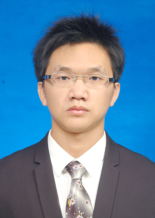
\includegraphics[width=1in,height=1.25in,clip,keepaspectratio]{yanyan.pdf}}]{Yan Yan}
received the B.Eng. degree and the MSc in Instrument Engineering at the Harbin Institute of Technology in 2010 and 2012 respectively. 
He worked as research assistance at the Shenzhen Institutes of Advanced Technology, Chinese Academy of Sciences from 2012 to 2014. 
He is working on his PhD in Computer Science started from 2014.
His research interests are digital signal processing, machine learning, and control system.
\end{IEEEbiography}

\begin{IEEEbiography}[]{Zhou Lin}
recived the B.Eng degree in Electronic information engineering at Wuhan University of Technology in 2014. she is studying for a master's degree at Wuhan university of technology from 2014 to now. Her research interests are digital signal processing and pattern recognition.
\end{IEEEbiography}

\begin{IEEEbiography}[]{Zhou Lin}
recived the B.Eng degree in Electronic information engineering at Wuhan university of technology in 2014. she is studying for a master's degree at Wuhan university of technology from 2014 to now. her research interests are digital signal processing and pattern recognition.
\end{IEEEbiography}

\begin{IEEEbiography}[{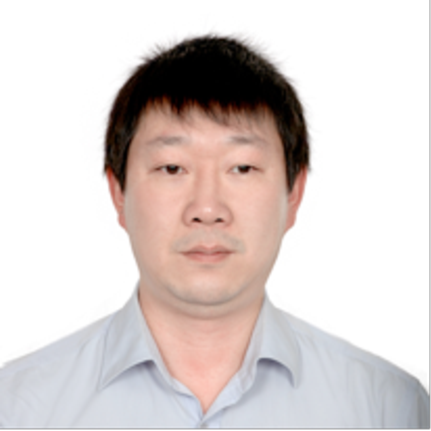
\includegraphics[width=1in,height=1.25in,clip,keepaspectratio]{wanglei.pdf}}]{Lei Wang}
received the B.Eng. degree in information and control engineering, and the Ph.D. degree in biomedical engineering from Xi’an Jiaotong University, Xi’an, China, in 1995 and 2000, respectively. He was with the University of Glasgow, Glasgow, U.K., and Imperial College London, London, U.K., from 2000 to 2008. He is currently a full professor with the Shenzhen Institutes of Advanced Technology, Chinese Academy of Sciences, Shenzhen, China. He has published over 200 scientific papers, authored four book chapters, and holds 60 patents. His current research interests include body sensor network, digital signal processing, and biomedical engineering
\end{IEEEbiography}


% insert where needed to balance the two columns on the last page with
% biographies
%\newpage

% You can push biographies down or up by placing
% a \vfill before or after them. The appropriate
% use of \vfill depends on what kind of text is
% on the last page and whether or not the columns
% are being equalized.

%\vfill

% Can be used to pull up biographies so that the bottom of the last one
% is flush with the other column.
%\enlargethispage{-5in}



% that's all folks
\end{document}


